\chapter{Literature Review}
\label{chap:lit_review}
This literature review is structured in the following way. Section \ref{section:lit:deduplication_in_hhs} kicks off with a discussion of a general framework on entity resolution, after which we review recent efforts aimed at deduplication of products from distinct Web shops. Section \ref{section:lit:introducing_lsh} continues by highlighting how and why \textit{locality-sensitive hashing} (LSH) has become one of the most important techniques in the field of entity resolution. Section \ref{section:lit:applying_lsh_to_deduplication_of_docs_on_web} expands on the previous section by highlighting specifically how LSH is applied to deduplication of entities found in the context of the Web and introduces the \textit{min-wise independent permutations locality-sensitive hashing} (MinHash) scheme. %The MinHash scheme is an example of an LSH family for the Jaccard similarity. 
Since the conception of the MinHash scheme, there have been many attempts to improve the effectiveness and scalability of Jaccard similarity LSH families such as the MinHash scheme. Therefore, we devote Section \ref{section:lit:variations_minhash} to an analysis of further developments related to Jaccard similarity LSH scheme. Lastly, in Section \ref{section:lit:amplifying} we discuss how LSH schemes can be improved further by discussing techniques such as amplification.

\section{Deduplication in Highly Heterogeneous Information Spaces}
\label{section:lit:deduplication_in_hhs}
As the Web has grown since its conception, its form and ways of use have been in a state of constant change. On the one hand, businesses, organizations, and individual users became much more prolific in producing new information to be displayed on the Web. On the other hand, the automatic extracting of information from raw data available on the Web became very accessible as technological tooling improved vastly. This caused a new sort of data space to come into existence: \textit{highly heterogeneous information spaces} (HHIS).

HHIS can be defined by a few key attributes. First, they contain non-structured data. This means that the schema of the data varies over the data points, which makes a structured comparison between these data points harder to perform. Second, the spaces are usually associated with high levels of noise. Especially when the addition of new data points highly relies on some form of user input, there is a large chance of missing data due to user errors, which in turn may lead to extraction errors. Last, it is important to mention that these spaces are generally very large. This means that any method, that aims to extract information or perform analyses, needs to be efficient.

In a very extensive effort, \cite{Papadakis2016} provide a discussion on the existing literature and methods in the field of \textit{entity resolution} (ER), which encompasses the challenge of finding items in datasets that relate to the same real-world entity. Within ER their efforts focus on the subclass Clean-Clean ER: the process of finding duos of matching items in two distinct, heterogeneous datasets, where each dataset is individually clean, which is a term that implies that there are no duplicates within the individual datasets. 

The authors review techniques that are related to data blocking. Data blocking techniques  group items in an entity set $E$ into blocks of data $B$. Detailed and often costly comparisons are only performed among the items contained within each block, so that all comparisons between items solely assigned to different blocks can be scrapped. Compared to the brute-force approach, which runs in quadratic time as each item needs to be compared to each other candidate item, these techniques provide a great increase in efficiency at the cost of some accuracy, since it may occur that a duplicate pair of items will not be contained in any of the blocks. LSH can be considered as a data blocking technique.

In order to be able to properly analyze the blocking techniques, the authors create a novel categorization. They argue that each blocking technique can be made up of at most three subtasks: the block building task, the block cleaning task and the comparison cleaning task.

The block building task takes as input two entity collections and generates blocks of potential duplicates. % This usually involves two key steps: the algorithm needs to extract so-called blocking keys. Based on the equality or similarity of blocking keys among items, items are placed in blocks. This usually involves a lot of redundancy so that a minimal number of potential duplicates are missed. 
The other two tasks are then applied to further reduce the number of comparisons in a way that is not too harmful to the performance of the algorithm. The block cleaning task aims to eliminate blocks which are constituted of a relatively high number of unnecessary comparisons. Comparison cleaning works on the more granular level of comparisons and is applied to each block. It aims to remove all unnecessary and redundant comparisons within the block.

The authors discuss and compare a total of $17$ methods that are made up of one or more of the subtasks discussed in the previous paragraph. It goes beyond the scope of this thesis to discuss all methods in detail. The optimal configuration of the methods is determined by maximizing the measure $\alpha(B,E) = RR(B,E) * PC(B,E)$. The \textit{reduction ratio} $RR(B,E)$ refers to the proportion of comparisons that is avoided by the blocking method. A high value of $RR(B,E)$ is associated with efficiency, since it lowers the amount of costly comparisons. The \textit{pair completeness} $PC(B,E)$ refers to the proportion of actual duplicates that occurs in at least one of the blocks. A high value of $PC(B,E)$ indicates that the method is very effective. Hence, by opting for a method that maximizes $\alpha(B,E)$, we obtain a method that strikes a balance between efficiency and effectivenes.

Further work on the specific problem at hand in this research has been carried out by \cite{DamGKNVF16}, who extend the \textit{multi-component similarity method} (MSM) first proposed by \cite{BezuBRVVF15}. MSM, an adapted single-linkage hierarchical clustering algorithm, has been shown to outperform other methods available at the time on identifying duplicate items among multiple sources. To achieve these results, the algorithm does have to make multiple costly passes over the data, hampering the potential scalability if the number of entities to be compared increases. This can happen if more sources come into play or the sources would start to contain more entities per source.

In an effort to improve the efficiency and scalability of the algorithm, the extensions by \cite{DamGKNVF16} entail the addition of an LSH scheme which can be interpreted as a relatively cheap block building method. Since it serves as a first step, this extension can also be seen as a preselection of suitable candidates. The result is a new method that is called the \textit{multi-component similarity method with preselection} (MSMP). 

In short, the application of the algorithm proceeds as follows: \textit{model words} are extracted from the title of the products. \textit{Model words} are defined as words that contain both numeric and non-numeric characters. The occurence of \textit{model words} in the title is used to create a binary vector $b_i$ for each item. This vector serves as input for the LSH scheme. The length of $b_i$ is equal to the cardinality of the set of all \textit{model words}. In each binary vector $b_i$, $b_{ij}=1$ represents the occurence of \textit{model word} $j$ in the product title of product $i$, while $b_{ij}=0$ is associated with its absence. LSH is then used to hash these binary vectors to buckets. The key idea of MSMP is that now MSM only needs to be applied to the elements within each bucket.  Depending on the specific tuning of the parameters of the LSH scheme, this will reduce the number of candidate duplicates by a large factor or by almost nothing. The authors show that a reduction of the pairwise comparisons by more than 80\% still results in a recall of duplicates of $0.8$, concluding that large computational advances can come at small performance decreases. 

Introducing the \textit{multi-component similarity method with preselection+} (MSMP+), \cite{HartveldKMNPFS18} aim to further improve the LSH step by extending the binary input vectors to also include model words extracted from the key-value pairs of the product inputs. Furthermore, a data cleaning step is added to increase the likelihood of a match on the \textit{model words}. These extensions lead to an increase of the \textit{area under the curve} (AUC) of the \textit{pair completeness} PC and \textit{pair quality} (PQ) by 12.2\% and 9.2 \%, respectively, compared to MSMP. 

It must be noted that the current implementation of LSH in MSMP+ still follows the original \textit{min-wise independent permutations locality-sensitive hashing} (MinHash) scheme by \cite{Broder00}. From this, one might conclude that there are further potential improvements, both computationally and performance-wise, to be made by implementing the more advanced proposals that have been made in the past two decennia. In order to gain a better understanding on the development of these LSH techniques, an in-depth discussion follows in the next section.

\section{The Path Towards Locality-Sensitive Hashing}
\label{section:lit:introducing_lsh}
In this section we first explain what problems LSH is aiming to solve. We then give a definition of LSH and discuss the relevance and influence of parameters that play a role in the LSH algorithm. 

To properly understand the circumstances and challenges under which LSH has been developed, we need to start with an introduction to the \textit{nearest neighbor problem} (NNP). One of the earliest discussions on NNP can be found in a book written by \cite{Minsky69}.%, who discuss the current state of solutions to a wide range of computation problems at the time. 
The version of NNP that the authors discuss is concerned with a dataset of $N$ words with a length of $b$ bits each. The authors focus on the challenge of finding a point $p$ in the data that is the \textit{best match} to an arbitrary query point $q$. The \textit{best match} is defined as the point $p$ that is closest to $q$ according to a pre-defined distance measure $D(p,q)$. 
%In order to analyze the memory and processing requirements of algorithms that tackle this problem, the authors look into methods that are split in two parts. The first part does the preprocessing of the items, in this case words with a length of $b$ bits, and stores a representation of the information in memory. The second part of the algorithm finds the solution to the problem and is only allowed to consider the information stored in memory by the first part. By using this structure, the authors are able to describe the impact of different levels of memory sizes and corresponding preprocessing costs on the computational cost of retrieving a \textit{best match}. 
The authors note that the related problem of finding an \textit{exact match} can be solved in reasonable time, as long as there is a sufficient amount of memory redundancy. In other words, if there is enough storage available, it is possible to create data structures that help to determine whether there is a point $p$ that is exactly equal to the input query $q$ and finding the location of $p$, and to do this efficiently. This result unfortunately does not transfer to the problem of finding the \textit{best match}. When the authors analyze this problem, they pose the conjecture that a very large amount of preprocessing and memory redundancy only leads to small speed-ups. For high-dimensional datasets of large scale the authors argue that the most optimal method is likely to be equivalent to brute-forcing, which comes down to doing a large search that goes through the majority of the memory, comparing the input $q$ to each point $p$ in the dataset. Although not offering a formal proof for this conjecture, the results of research in the decennia to follow turned out to confirm this belief.

In a seminal paper \cite{IndykM98} note that, after decades of further research, optimal solutions to NNP in high-dimensional spaces are still marginally better than the brute-force algorithm mentioned in the previous paragraph. In order to advance the literature on this topic, they shift their focus to a slightly redefined version of the original problem, which is known as the \textit{$\epsilon$-approximate nearest neighbour problem} ($\epsilon$-NNP).

In this version of the problem we are interested in finding the $\epsilon$-approximate nearest neighbor of an arbitrary query point $q$ in a set of $n$ points $P = {p_1,...,p_n}$, where the $\epsilon$-approximate nearest neighbor is defined as the point (or set of points) that is within $(1 + \epsilon) * d$ distance of $q$, where $d$ refers to the distance of $q$ to the true nearest neighbor in $P$. For reasonably small values of $\epsilon$, solutions to this relaxed version of the problem should still suffice for most practical purposes of similarity search, especially taking into account that the notion of similarity itself is not necessarily a mathematically very rigorously defined concept in general. At the time of writing, solutions to the $\epsilon$-NNP were dealing with the same limitations as the original problem. 

In the same paper, \cite{IndykM98} introduce LSH as a solution to the $\epsilon$-NNP. Not surprisingly considering the naming, LSH relies on the use of hash functions. Hash function are functions that generate fixed-size outputs from arbitrary-sized inputs. Till then most applications of hash functions, such as in cryptographic hashing, relied on hash functions having a near-zero probability of colliding for two arbitrary, different inputs. The contrary is the case for LSH, which relies on the use of hash functions for which the probability of collision is much higher for inputs $p$, $q$ that are closer together according to a metric $d(p,q)$ defined on the space $P$. They provide the following proper definition of a locality-sensitive family of hash functions:
\begin{definition}\label{def:LSH}
    A family $\mathcal{H} = {h: P\rightarrow U} $ is called $(d_1, d_2, p_1, p_2)$-sensitive if for any $x,y \in P$ and $h$ chosen uniformly from $\mathcal{H}$ satisifies the following properties:
\begin{itemize}
    \item if $\operatorname{sim}(p, p') \geq d_1$ then $\operatorname{Pr_{\mathcal{H}}}[h(p)=h(p')] \geq p_1$
    \item if $\operatorname{sim}(p, p') \leq d_2$ then $\operatorname{Pr_{\mathcal{H}}}[h(p)=h(p')] \leq p_2$
\end{itemize}
\end{definition}
In the definition above, $U$ refers to the space that contains all hashes that potentially result from the hash functions $h$.
\cite{IndykM98} show that if such a locality-sensitive family of hash functions $\mathcal{H}$ exists for the (dis)similarity measure of interest $\operatorname{sim}(\cdot, \cdot)$, this family can be used to construct a method that under the correct circumstances solves the $\epsilon$-NNS problem in sublinear time. More specifically, such an algorithm uses $O(dn + n^{1+\rho})$ space and $O(n^{\rho})$ evaluations of the hash functions for each query $q$, where $\rho = - \frac{\log{p_1}}{\log{\frac{p_1}{p_2}}} = - \frac{\log{p_1}}{\log{p_1} - \log{p_2}}$.

\begin{equation}
    \begin{aligned}
    \frac{\partial \rho}{\partial \log{p_1}} &= - \frac{(\log{p_1} - \log{p_2}) -\log{p_1}}{(\log{p_1} - \log{p_2})^2} = \frac{ \log{p_2}}{(\log{p_1} - \log{p_2})^2} \\
    \frac{\partial \rho}{\partial \log{p_2}} &= - \frac{\log{p_1}}{(\log{p_1} - \log{p_2})^2} = - \frac{ \log{p_1}}{(\log{p_1} - \log{p_2})^2}
    \end{aligned}
    \label{eq:partial_derivatives_rho}
\end{equation}
Under the restriction that $0 < p_2 < p_1 < 1$, we know that $\log{p_2} < \log{p_1} < 0$, so that $(\log{p_1} - \log{p_2})^2 > 0$. It then follows that $\frac{\partial \rho}{\partial \log{p_1}} < 0$ and $\frac{\partial \rho}{\partial \log{p_2}} > 0$. Thus, one might note that as $p_1$ and $p_2$ lie further apart ($p_1 \rightarrow 1$, $p_2 \rightarrow 0$), the algorithm becomes increasingly more efficient ($\rho \rightarrow 0$). 

In short, the algorithm proceeds as follows. We define a function family $\mathcal{G} = {g: P\rightarrow U^k}$ such that $g(p) = (h_1(p),...,h_r(p))$, where $h_i\in\mathcal{H}$. Then we randomly draw $b$ independent functions $g_1,...,g_b$ from $\mathcal{G}$. For each item $p$ in our collection $P$ and for $j=1,...,b$, we compute $g_j(p)$. Now, if $g_j(p)=g_j(p)$ for some $j\in{1,...,b}$ and $p,p'\in P$, then we say that $p$ and $p'$ are assigned to the same bucket $g_j(p)$, which in its essence is nothing more than a hashcode. We can use this fact to construct a hash table, which allows us to efficiently look for points that are close to arbitrary input points $q$. 

\cite{Charikar02} offer an alternative definition of an LSH scheme to \cite{IndykM98}, but the underlying idea and resulting applications are the same:
\begin{definition}
A locality-sensitive hashing scheme refers to a distribution on a family $\mathcal{H}$ of hash functions operations on a collection of objects, such that for two objects $x$,$y$,
\begin{equation*}\label{def:LSH_2}
    \operatorname{Pr}_{h \in \mathcal{H}}[h(x)=h(y)]=\operatorname{sim}(x, y)
    \end{equation*}
where $\operatorname{sim}(x, y)$ is some similarity function defined on the collection of objects.
\label{def:lsh_charikar}
\end{definition}

A similarity function $\operatorname{sim}(x,y)$ is intended to capture the similarity between entities $x$ and $y$. The output of the function is between $0$ and $1$. A value close to $0$ implies that the entities are very different, while a value close to $1$ means that the entities are nearly identical.
\cite{Charikar02} establishes various conditions that the similarity function needs to adhere too in order for a corresponding LSH scheme to exists. Most importantly, he shows that, if a similarity function $\operatorname{sim}(x,y)$ admits an LSH scheme as defined in Definition \ref{def:lsh_charikar}, then the distance function $1 - \operatorname{sim}(x)$ must adhere to the triangle equality. More specifically, for any $x,y,z \in X$, where $X$ denotes the metric space of interest, we have
\begin{equation}
    1 - \operatorname{sim}(x,y) \leq (1 - \operatorname{sim}(x,z)) + (1 - \operatorname{sim}(y,z))
\label{eq:triangle_inequality}
\end{equation}

Using this established fact, the author proves that there is no LSH scheme for a number of similarity functions that are popular in the field of information retrieval, such as Dice's coefficient and the Overlap measure. The Jaccard similarity, which plays a large role in Section \ref{section:minhash}, does adhere to these conditions.

It is of importance to note the influence of the parameters $b$ and $r$. $b$ denotes the number of buckets each point $p$ is assigned to. A higher value for $b$ thus results in a higher chance of collision for arbitrary points $p$ and $p'$. $r$ denotes the number of hash functions $h_i(\cdot)$ that need to agree for points $p$ and $p'$ such that they are assigned to the same bucket. Hence, a higher value for $r$ leads to a lower chance of collision for $p$ and $p'$. Whenever a LSH scheme is implemented, the practitioner needs to decide on appropriate values for $b$ and $r$. 

We can actually express the probability that there is a match between two entities $p$ and $p'$ in a formula, wich depends on the actual similarity $s(p,p') = s$, $b$, and $r$. We know that the probability of a single element in two sketches being equal, $\operatorname{Pr}[h_i(p) = h_i(p')]$, is equal to $s$.  The hash functions $h_i\in\mathcal{H}$ are independent, which implies that $\operatorname{Pr}[h_i(p) = h_i(p'), \forall i \in \{1,...,r\}] = s^r$ for every $g_j(p)$. Hence, the probability, that there is no $j \in \{1,..,b\} : g_j(p)=g_j(p')$, is equal to $(1- s^r)^b$. As probabilities must sum to $1$, the probability that there is at least one bucket $g_j(p)$ to which $p'$ is assigned as well, which makes $(p, p')$ a candidate pair, is then given by the following formula

\begin{equation}
    \operatorname{Pr}[g_j(p)=g_j(p') \text{ for some } j\in{1,...,b}] = 1 - (1-s^r)^b
    \label{eq:s_curve}
\end{equation}

The formula in Equation \ref{eq:s_curve} is usually referred to as the s-curve. From an analysis of the s-curve we can reach the same conclusions with respect to the effects of parameter changes as earlier. If we keep $s$ constant, we see that an increase of $b$ would lead to a larger chance of $p$ and $p'$ sharing at least one bucket, as $1-s^r < 1$. For $r$, we see that an increase would have an opposite effect, where the chance of $p$ and $p'$ colliding in a bucket will actually decrease. In figure \ref{fig:multiple_s_curves} we have plotted the s-curve for several settings of $b$ and $r$, conditional on the number of hash functions $h_i(p)$ used being equal to $256$. 

\begin{figure}
    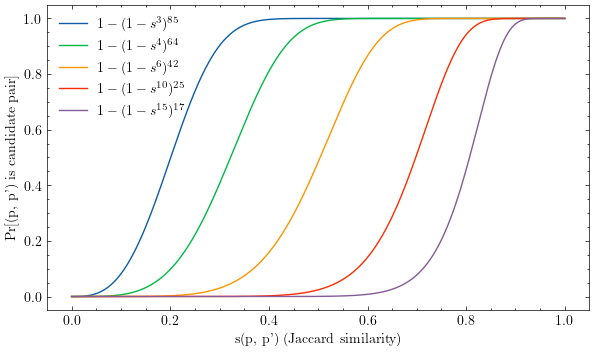
\includegraphics[width=\textwidth]{multiple_s_curves_without_threshold.png}
    \caption[Plot of several s-curves]{\textbf{Plot of several s-curves}. The plot shows the form of the s-curve for different settings of $b$ and $r$. The number of hash functions $n$ used is $256$.}
    \label{fig:multiple_s_curves}
\end{figure}

How do we find optimal values for $b$ and $r$? To answer this question, it helps to take into account the goal of applying LSH, which, in the context of this research, is to find all points $p,p' \in P$ that are likely to be close together according to some similarity metric $\operatorname{sim}(p, p')$. As $\operatorname{sim}(p, p')$ increases, $\operatorname{Pr}[(p,p') \text{is a candidate pair}]$ increases as well. This speed of increase is not constant: It starts out small and grows until a certain maximum level, after which it declines again. The point at which the maximum level is reached, which is the steepest part of the s-curve, is generally referred to as the threshold $t$. This is the point where an increase in $\operatorname{sim}(p, p')$ has the biggest impact on the chance that $p$ and $p'$ are a candidate pair. It tends to coincide with $\operatorname{Pr}[(p,p') \text{is a candidate pair}] = 0.5$. It is obvious that a change in $t$ would affect parameters $b$ and $r$, but how can we formalize this relationship?

Since $t$ occurs at the steepest part of the s-curve, we can relate $t$ to $b$ and $r$ by solving

\begin{equation}
    \frac{\partial^2 1 - (1-s^r)^b }{\partial s^2} = 0
    \label{eq:identifying_equation}
\end{equation}

It turns out that the threshold $t$ depends on $r$ and $b$ according to Equation \ref{eq:threshold_equation}. Derivations to arrive at this result have been placed in Appendix \ref{appendix:derivation_threshold}.

\begin{equation}
    t = (\frac{r-1}{rb-1})^{\frac{1}{r}} \simeq (\frac{r}{rb})^{\frac{1}{r}} = (\frac{1}{b})^{\frac{1}{r}} \text{ for } r,b \gg 1
    \label{eq:threshold_equation}
\end{equation}

Together with the constraint that the maximum of $r * b$ is equal to the number of hash functions $n$ that we use, we can use equation \ref{eq:threshold_equation} to calculate suitable values of $r$ and $b$ for any choice of $n$ and $t$. 

\begin{figure}
    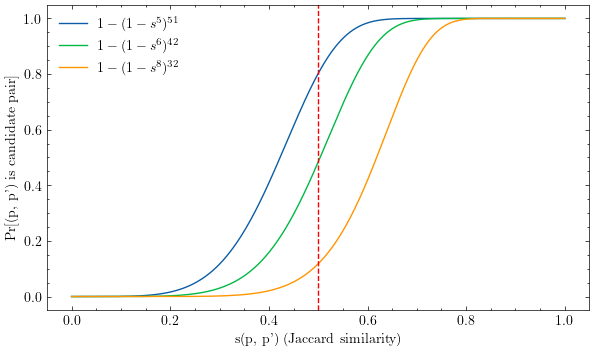
\includegraphics[width=\textwidth]{multiple_s_curves_with_threshold.png}
    \caption[Plot of several s-curves with threshold]{\textbf{Plot of several s-curves with threshold}. The plot shows the form of the s-curve for different combinations of $b$ and $r$. The number of hash functions used is $256$. The red line indicates a threshold value of $0.5$}
    \label{fig:multiple_s_curves_with_threshold}
\end{figure}

A second approach for determining $r$ and $b$ is found in an article by \cite{ZhuNPM16}. We present their approach below. In Figure \ref{fig:multiple_s_curves_with_threshold} we plot a selection of s-curves and add a line at $s(x,y) = 0.5$, which represents a threshold value of $0.5$. Given this threshold, what arguments could be given in favour of each s-curve and corresponding parameter configuration? For the blue line described by the formula $1 - (1-s^5)^{51}$, we find that on a relatively large range of values of $s(x,y) < 0.5$ a positive probability of declaring $(x, y)$ a candidate pair. In other words, the number of false positives is higher compared to the green and orange line. On the other hand, for values of $s(x, y) > 0.5$ the blue line converges to $1$ sooner than the other two line, which implies that the number of false negatives is lower. By the same line of reasoning, we can see that the orange line provides a very low number of false positives, but a relatively large number of false negatives. In general, given specific values of $b$ and $r$, we can define the probabilities of false negatives and false positives in case of a threshold of $0.5$ as follows:

\begin{equation}
    \begin{split}    
        \operatorname{Pr}[\text{False positive}] &= \operatorname{Pr}[(x, y)\text{ is a candidate pair}| s(x, y) < 0.5 ] = \int_{0}^{0.5}1 - (1-s^r)^bds \\
        \operatorname{Pr}r[\text{False negative}] &= \operatorname{Pr}[(x, y)\text{ is not a candidate pair}| s(x, y) > 0.5 ] = \int_{0.5}^{1}(1-(1 - (1-s^r)^b)ds
    \end{split}
\end{equation}

\begin{figure}
    \centering
    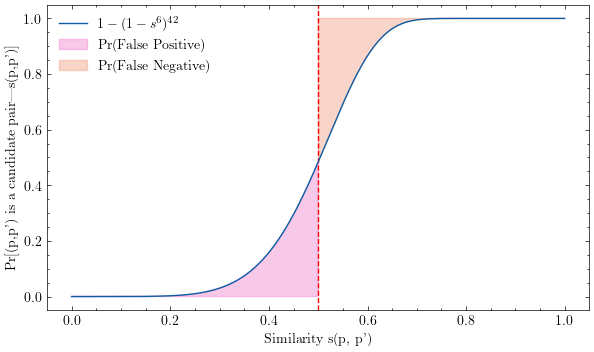
\includegraphics[width=0.75\textwidth]{error_s_curve_t05_n_256.png}
    \caption[Plot of several s-curves]{\textbf{Plot of several s-curves}. The plot shows the relation between the form of the s-curve on one hand and $\operatorname{Pr}[\text{False positive}]$ and $\operatorname{Pr}[\text{False negative}]$ on the other hand. }
    \label{fig:s_curve_with_fn_fp}
\end{figure}

These probabilities are graphically represented in figure \ref{fig:s_curve_with_fn_fp}. The pink tinted area corresponds to the probability of false positives, while the orange tinted area is equivalent to the probability of false negatives. Depending on the application, users might place more value on preventing false negatives than preventing false positives or vice versa. These preferences can be accomodated in the choice of values of $b$ and $r$ by minimizing the weighted average of $\operatorname{Pr}[\text{False positive}]$ and $\operatorname{Pr}[\text{False negative}]$ for a certain threshold $t$ with respect to $b$ and $r$. This comes down to solving the following problem

\begin{equation}
    \argmin_{b,r} w_{FP} * \int_{0}^{t}1 - (1-s^r)^bds + w_{FN} * \int_{t}^{1}(1-(1 - (1-s^r)^b)ds
    \label{eq:optimize_for_b_and_r}
\end{equation}

We can vary the weights to indicate a change in our preferences. A relatively larger value for $W_{FP}$ indicates that we would rather prevent false positives than false negatives, while a relatively larger value for $W_{FN}$ would indicate an opposing preference. While not necessary, it is a good custom to let the sum of $W_{FN} + W_{FP}$ equal $1$. 

\begin{figure}[!htb]
    \centering
    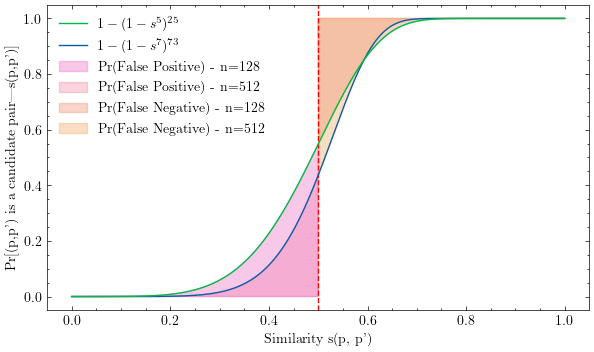
\includegraphics[width=0.75\textwidth]{error_s_curve_t05_n_512_128.png}
    \caption[Effect of change of $n$ on s-curve]{\textbf{Effect of change of $n$ on s-curve}. Plot of s-curves showing the effect of an increase of $n$ on $\operatorname{Pr}[\text{False positive}]$ and $\operatorname{Pr}[\text{False negative}]$  }
    \label{fig:change_in_s_curve_as_n_increases}
\end{figure}

Figure \ref{fig:change_in_s_curve_as_n_increases} shows what happens to $\operatorname{Pr}[\text{False positive}]$ and $\operatorname{Pr}[\text{False negative}]$, if we increase the number of hash functions $n$ from $n=128$, associated with the green s-curve, to $n=512$, associated with the blue s-curve. A higher value of $n$ allows $b$ and $r$ to become larger, which changes the form of the s-curve. If one would continue to increase $n$, we eventually arrive at a s-curve with the form of a step function: For all values $s(p, p')$ lower than the threshold $t$ the probability of being a candidate pair would be $0$, while this would be $1$ for all values $s(p, p')$  greater than $t$.  


\section{Applying LSH to Deduplication Problems Related to the Web}
\label{section:lit:applying_lsh_to_deduplication_of_docs_on_web}
After explaining what LSH entails in the previous section, this section continues by explaining how LSH, and specifically the MinHash sketching scheme, has become a prominent technique to apply to deduplication of entities. 

After its conception in 1989 by Sir Tim Berner-Lee, the World Wide Web immediately started to grow at a massive pace. The first Web browser and website became available in 1990 and just $6$ years later, the number of websites available surpassed $1$ million\footnote{data retrieved from https://www.internetlivestats.com/total-number-of-websites}. This exponential increase in use and creation of webpages also created a new application for the field of similarity search. Webpages in their most basic form are essentially just documents, structured collections of letters, words, and sentences. Often, these documents would be reused in different locations on the Web. For users to have a good experience on the Web, it would be required that search engines do not return the same page from different domains on the same search query. Hence, it became of increasing relevance to create effective deduplication methods. 

A first attempt at solving this probem is done by \cite{Broder97}, who tackles the challenge of identifying (nearly) identical documents. The author notes that distance measures defined on strings developed up to that time, such as the Hamming and Levenshtein distance, are not suitable for the comparison of entire documents. To capture the informal notion of two documents that are ``roughly the same'', he defines a resemblance measure $r(A,B)$. This measure is a number between 0 and 1 and should be closer to 1 if the document $A$ and $B$ are more likely to be the same. An attractive property of his proposed measure is that the resemblance distance, defined as $d(A,B) = 1 - r(A,B)$, is a metric (distance measure). In general, $r(A,B)$ is implemented by extracting elements from $A$ and $B$ and counting the number of shared elements between $A$ and  $B$, mathematically defined as $\vert A \cap B \vert$. We then let $r(A,B) = \frac{\vert  A \cap B  \vert}{\vert A \cup B \vert }$. This is a well-known measure in literature called the Jaccard similarity \citep{jaccard1912distribution}. But how does one define the elements in $A$ and $B$ with respect to documents?

To this end, \cite{Broder97} comes up with the notion of shingles. A shingle is a subsequence of tokens contained in the document, where tokens can be either letters, words, or entire lines. The \textit{w-shingling} is then defined as the bag of all shingles with length $w$ that can be extracted from a document. By dividing the size of the intersection of the two bags by the size of the respective union, the overlap between the documents can be quantified, which leads to the resemblance measure $R(A,B)$. As the calculation of all resemblance measures $r(A,B)$ over a set $ \{(A,B) : A,B \in D, \vert D \vert = n\}$, where $D$ refers to the set of all bags of shinglings, runs in quadratic time $O(n^2)$, the author looks into methods that can estimate the resemblances more efficiently.

The resemblances are estimated by using a sampling process that generates fixed-size sketches of each document. From here on, let $[n]= {0,1,...,n-1}$. As a start, each shingle is assigned a unique id of $m$ bits, so that the total number of available ids is equal to the size of $[2^m]$. A random permutation $\pi$ on $[2^m]$ is defined and applied to each bag of shingles. For each document, the ids of the shingles that are mapped to the smallest $s$ values according to the new permutation are kept and will form the so-called \textit{fingerprint} of the document. %The fixed-size fingerprint is then created by iteratively generating randomly permutations $\pi$ on the set ${1,2,...,2^l}$ and storing the resulting minimal coefficient for each document.

These sketches can then be used to estimate the resemblance between documents by applying the Jaccard similarity measure: The estimated resemblance between two documents is equal to the number of elements shared between the two sketches divided by the size of the union of the elements in the sketches. 
% The sampling process that generates the sketches runs in linear time ($O(n)$). Since the time to compute the sketch 
Since the sampling process that generates the sketches runs in linear time ($O(n)$), this method can greatly reduce computational costs associated with identifying (nearly) identical documents.
% Using this method, the job of clustering a batch of $n$ documents into sets of documents, which closely resemble each other, runs in $O(n \log n)$ time instead of $O(n^2)$. 

In order for the algorithm above to work, we need a random permutation $\pi$ of a large set of integers ${0,...,...,2^{m}-1}$, with $m$ sufficiently large. Obviously, when determining a proper value of $m$ there is a trade-off between the chance of collision, which should be minimalized, and the cost of storage. The author proposes to use Rabin fingerprints \citep{Rabin1984} for generating the ids of the shingles, since the probability of collision is well understood and implementation in software is very efficient. 

\subsection{MinHash}
In a subsequent effort, \cite{Broder00} take the key ideas of their previous paper and describes the method that has come to be known as MinHash. Rabin fingerprints are used to generate a set of ids $S_D$ that represent each document $D$. Contrary to the earlier proposal, which only used one permutation, a set of $n$ independent random permutations $\pi_1,\pi_2,...,\pi_n$ is chosen. The sketch of each document $D$ is now defined as 
\begin{equation}
    \operatorname{sketch}_D = (\min\{\pi_1(S_D)\}, \min\{\pi_2(S_D)\},...,\min\{\pi_n(S_D)\})
\end{equation}

Now the resemblance between documents $A$ and $B$ can be estimated by counting the number of shared elements in their respective sketches. This follows from the fact that, under certain conditions on the random permutation function $\pi$
\begin{equation} \label{eq:MinHash}
    \operatorname{Pr}[\min\{\pi(S_A)\} =  \min\{\pi(S_B)\}] = \frac{|S_A\cap S_B|}{|S_A\cup S_B|} = r(A,B)
\end{equation}
One might note the similarity of Equation \ref{eq:MinHash} to the definition of LSH in Equation \ref{def:lsh_charikar}. Indeed, the MinHash function $h_i(x) = \min\{\pi_i(x)\}$ is a valid hashing function in a LSH scheme for the Jaccard similarity function $r(A,B)$ as defined by \cite{IndykM98} and \cite{Charikar02}.

A more in-depth discussion on conditions, that the random permutation function $\pi$ needs to adhere to in order to validate Equation \ref{eq:MinHash}, is proposed by \cite{DBLP:journals/jcss/BroderCFM00}. The authors note that many algorithms that use hash functions assume that these functions are truly random, an assumption which is practically impossible to meet in practice. Nonetheless, the authors argue that for the algorithm described in the previous paragraph a less strict assumption is required, which is that the permutation $\pi$ needs to be drawn from a min-wise independent family of permutations.

A family $F\subseteq S_u$, where $S_u$ denotes the set of all permutations on $[u] = {0,1,...,u-1}$, is said to be min-wise independent if all elements $x$ in a set $X \subseteq [u]$ that are permuted by a random permutation $\pi \in F$ have an equal probability of being the minimum element. More formally, we have 
\begin{equation}
    \operatorname{Pr}[min\{\pi(X)\}=\pi(x)] = \frac{1}{|X|}
\end{equation}
% If $n$ is too large, it becomes impossible to define such families. Hence, in practice smaller families of permutations are considered.

In practice, instead of generating and storing $n$ random permutations of length $u$, MinHash is implemented by randomly choosing $n$ hash functions $h(x)$ from a universal family of hash functions. A universal hash function $h:[u]\rightarrow[u]$ has the attractive propery that the probability of collision for two inputs $x$, $y$ ($x\neq y$) is smaller than $\frac{1}{u}$. \cite{CarterW79} propose the following, still widely used universal hash function applicable to integer inputs.
\begin{equation}
    h(x) = ((a * x + b) \bmod p) \bmod u
    \label{eq:universal_hashing}
\end{equation}
where $a$ and $b$ are random integers chosen from $[p] = \{0,1,...,p-1\}$ and $p$ is a prime. A  popular choice for $p$ is a mersenne prime, a prime as close as possible to a power of $2$, such as $2^{61} - 1$. 
% This allows for an efficient implementation of the hash function where the $\bmod p$ operation only requires applying bitwise operators and shifts to $(a*x + b) $ and $p$. 
%The hashing function in (\ref{eq:universal_hashing}) even possesses the stronger uniform property, which says that for $x\neq y$ the difference $h(x) - h(y)$ is uniformly distributed on $[n]$. 

% \subsection{Random Projection (SimHash)}
% On a first look, one would argue that this is also the case for the cosine similarity, which is a popular similarity measure usually applied to vectors in Euclidean space. The cosine similarity solely depends on the angle between two vectors. It is particulary useful when comparing vectors extracted from a sparse space, since only the non-zero values are necessary for calculating the similarity. Mathematically, the cosine similarity is defined as follows:
% \begin{equation}
%     \operatorname{sim}(x,y)  = \frac{x^ty}{\lVert{x}\rVert_2 \lVert{y}\rVert_2 }
% \end{equation}
% The output will always be in $[-1,1]$. Using a counterexample, it is straightforward to show that the corresponding distance function does not adhere to the triange inequality. Hence, it is not possible to define a locality sensitive hashing family for the cosine similarity. 

% The author devises the following, remarkably simple hashing scheme that is strongly related to the cosine similarity. It works by drawing a random vector $r$ from the $d$-dimensional Gaussian distribution. Then the corresponding hash function is defined as 
% \begin{equation}
%     h_{r}(x)= \begin{cases}1 & \text { if } r \cdot x \geq 0 \\ 0 & \text { if } r \cdot x<0\end{cases}
%     \end{equation}
% It can then be shown that
%     \begin{equation}
%         \operatorname{Pr}\left[h_{r}(x)=h_{r}(y)\right]=1-\frac{\theta(x, y)}{\pi} = 1 -  \frac{1}{\pi} \cos^{-1}(\frac{x^{t}y}{\lVert{x}\rVert_2 \lVert{y}\rVert_2})
%         \end{equation}
%where $\theta = \cos^{-1}(\frac{\mathbf{x}_i^t\mathbf{x}_j}{\lVert\mathbf{x}_i\rVert_2 \lVert\mathbf{x}_j\rVert_2 }$. 
% Although this function, in most papers referred to as the angular similarity, is not exactly the same as the cosine similarity, it is obvious that the two are closely related. Since $\theta(x, y) = \cos^{-1}(\frac{x^{t}y}{\lVert{x}\rVert_2 \lVert{y}\rVert_2 })$ and $\cos^{-1}(x)$ is a monotonically decreasing function on $x \in [-1,1]$, we know that $1 - \frac{\theta}{\pi}$ is monotonically increasing with respect to the cosine similarity. In the remainder of this paper we refer to the Random Projection method as SimHash.
%\cite{GoemansW95} show that this use of the random hyperplane technique implies that the result is always at least a factor 0.878 or higher from the cosine similarity, hence the close relationship. 
% In the same paper \cite{Charikar02} propose a method for finding the $k=1$ $(1+\epsilon)$-approximate nearest neighbor of an arbitrary element in a collection that only requires traveling $O(n^{\frac{1}{1+\epsilon}})$ elements.
%\subsection{Kernelized Locality-Sensitive Hashing}

%\cite{KulisGrauman12} extend the random hyperplane technique to problems where only the result of kernel functions is known and underlying embeddings of the data are not known. Mostly useful in the case of comparing visual representations. 

\section{Experimenting with alternatives for MinHash}
\label{section:lit:variations_minhash}
In the previous section we have laid down how the MinHash LSH scheme is constructed and used in daily practice. This section is devoted to efforts that have been focussed on further refining and developing LSH schemes related to the Jaccard similarity.

Although MinHash was introduced as a technique to increase the efficiency of deduplication algorithms, the original implementation still requires an expensive preprocessing step, in which a number of random permutations $t$ on the data need to be computed. Multiple alternatives have been formulated that aim to decrease the number of required permutations and to potentially increase the accuracy of the estimates.

\cite{LiCH06} devise a method called \textit{conditional random sampling} (CRS), in which the first $k$ non-zero entries from a random permutation on the data are used to estimate the pairwise distance or inner product of data points. This method is quite similar to the original sketching proposal by \cite{Broder97}, but cannot be used in a LSH scheme, since there is no guarantuee for the length of the resulting sketch, if there are less than $k$ non-zero entries for a data point.

\subsection{One permutation hashing}

\cite{Ping2012} propose a method called \textit{one permutation hashing} (OPH) which, not surprisingly taking into account its name, only requires one permutation on the data to provide estimates of the Jaccard similarity between items in the dataset. The main idea here is to divide the permuted data in bins of equal length. The hashes are the result of extracting the location of the first non-zero element within each bin. It might happen that a bin only contains zero-valued elements. Such (empty) bins are denoted by $*$. The estimate of the Jaccard similarity $\hat{R}$ between vectors $x_i, x_j$ is then given by 
\begin{equation}
    \hat{R} = \frac{N_{mat}(i,j)}{k-N_{emp}(i,j)}
\end{equation}
where $N_{mat}(i,j)$ refers to the number of jointly matching bins, $N_{emp}(i,j)$ refers to the number of jointly empty bins and $k$ refers to the total number of bins. The authors show that $\hat{R}$ is an unbiased estimator of the Jaccard similarity. When the data is  sparse, the chance of empty bins is high. This makes it hard to use this hash function in an LSH scheme, since hashes from two inputs $p$ and $p'$ cannot be aligned if an empty bin occurs in one of the two hashes. The occurence of empty bins also decreases the preciseness of the estimate of the similarity between the two inputs.
% A high number of empty bins also impacts the preciseness of the estimate. 

\cite{Shrivastava014densified} extend OPH by adding a \textit{rotation} step: If an empty bin occurs, the value is replaced by the hashed value of the next non-empty bin.
%with an added offset value of $tC$, where $C = \frac{D}{k} + 1$ is a constant and $t$ is the number of steps that are necessary in the rotation. 
The underlying idea is that for each input $p$ the positions of empty and non-empty bins are random, so that the reassignment comes down to randomly re-using the existing hashes. Hence, the resulting hash function satisfies the LSH property in Definition \ref{def:LSH_2}. 
% They show that regardless of data sparsity or number of bins $k$ the resulting estimator is unbiased with respect to the resemblance, thus fixing the defects of the original OPH estimator. In empirical tests on nearest neighbor search problems, the estimator performs on par with the original MinHash scheme, while operating at a fraction of the computation costs.

%WHY DOES RANDOMNESS HELP?
In a paper written in the same year as the one cited in the previous paragraph, \cite{Shrivastava014Improved} expand on these results and suggest an improved densified OPH estimator. % Instead of always going right or left, this new scheme assigns to each bin $i$ a i.i.d. Bernouli random variable $q_i$ which decides the direction of choice in the case of bin $i$ being empty. If bin $i$ is not filled, the algorithm has a look at $q_i$. If $q_i = 1$, then the first non-zero entry to the right comes into play. If $q_i = 0$, we select the first non-zero entry to the left as our replacement value. It turns out that this addition of extra randomness improves the performance of the estimator: the authors argue that the theoretical variance of their new estimator is lower than their previous proposal, which should lead to a better precision in practice. This is confirmed by their experiments.
In an application to the estimation of resemblance of words based on co-occurence in documents, the improved scheme delivers a lower \textit{Mean Square Error} (MSE) for larger values of $k$ and for relatively more sparse inputs compared to the method proposed by \cite{Shrivastava014densified}. Unfortunately, as $k$ grows, the variance of the newly proposed estimator does not converge to $0$, but to a positive constant. 

Another, more recent iteration on densification schemes has been carried out by \cite{Shrivastava17}.The author notes that the key to further reduction of the variance for larger values of $k$ is to increase the randomness in the replacement process for empty bins. To achieve this, the author turns his attention to the concept of $2$-universal hash functions, which are functions that for different inputs assign an equal probability to each combination of outputs that is in the range of the function. % When the algorithm stumbles upon an empty bin, such a hash function is used to generate indices, until an index is found to which a non-empty bin is associated. The value of this bin is then used as the value for the original empty bin. In order to prevent the occurence of cycles, the number of attempts is taken as a second argument to the hash function. For a full description of the algorithm we refer to the original paper. 
The ``optimal'' densified estimator, as the author likes to call it, achieves a variance that is drastically superior to the variance of previous densified OPH estimators, especially when a large number of bins is used or the data is very sparse. 
% In an experimental setting it achieves these results 10-18 times faster than MinHash.

\subsection{Fast simimilarity sketching}
\label{subsec:fss}
\cite{DahlgaardKT17} propose a method, which they name \textit{fast similarity sketching} (FSS). % that is supposed to combine the best characteristics of both the original MinHash method as well as the later OPH methods. 
FSS can be understood as a combination of \textit{sampling with replacement}, taking inspiration from MinHash, and \textit{sampling without replacement}, which is found in OPH. Thus, the authors claim that FSS combines the best characteristics of MinHash and OPH. The sketching method takes as input a set of distinct integers $p \subseteq [u] $, where $[u]$ is defined as $\{0,1,...,u-1\}$. The output of the algorithm is a sketch $S(p)$ of size $n$. 

The detailed implementation works as follows. For all elements $a \in p$, we define a total of $2n$ random hash functions $h_i(a) = (b_i(a), v_i(a))$, where $b_i(a)$ refers to the index of a bin in $S(a)$ and $v_i(a)$ refers to the value that is placed in the bin. Depending on the value of $i$, $b_i(a)$ and $v_i(a)$ are restricted in the following ways,
\begin{equation}
\begin{aligned}
    &h_i: [u] \rightarrow [n] \times [i, i + 1)  & \text{ if } i \in [n] \\
    &h_i: [u] \rightarrow \{i-n\} \times [i, i + 1)  & \text{ if } i \in \{n,...,2n-1\}
\end{aligned}
\label{eq:random_hash_functions_fss}
\end{equation}
In other words, for $i \in [n]$, $b_i(a)$ maps to a random integer value in $[n]$. If $i \geq n$, $b_i(a)$ is guaranteed to be equal to $i-n$. In all cases, $v_i(a)$ is equivalent to a random real value in $[i, i + 1)$. Following these restrictions on the random function hash functions $h_i(a)$, the $j$th entry of $S(p)$ is defined as follows:
\begin{equation}
    S(p)_j = \min \{v_i(a) | a \in p, i\in [2n], b_i(a)=j\}
    \label{eq:definition_sketch_fss}
\end{equation}
%Put into words, the $j$th entry of $S(A)$ is equal to the index $i$ of the first hash function $h_i(a)$ where the first part of the  output is equal to $j$.
% The hash functions $h_n,...,h_{2n-1}$ make a second pass over the sketch, ensuring that all entries of $S(p)$ are properly defined. %maybe put somewhere else?

The authors present the fill-sketch algorithm, which efficiently generates the sketch $S(p)$ as defined in Equation \ref{eq:definition_sketch_fss}. See Algorithm \ref{alg:fill_sketch_algorithm} for pseudo code detailing the implementation of the Fill-sketch algorithm.

\begin{algorithm}
    \KwData{\\
    $p$: Set of inputs $a$ from which sketch needs to be created 
    }
    \KwIn{\\
    $n$: Length of sketch \\
    $h_0,...,h_{2n-1}$: Random hash functions }
     
\KwResult{The sketch $S$}
$S \gets \infty^n$\;
$c \gets 0$\;
\For{$i = 0;\ i < 2n;\ i = i + 1$}{
    \For{$a \in p$}{
        $v, b \gets  h_i(a)$\;
        \If{$S[b]=\infty$} {
            $c \gets c + 1$\;
        }
        $S[b] \gets \min(S[b],v)$\;
    }
    \If{$c=n$}{
        \KwRet{$S$}
    }
}
\caption{Fill-sketch algorithm}
\label{alg:fill_sketch_algorithm}
\end{algorithm}

\begin{figure}[!htb]
    \centering
    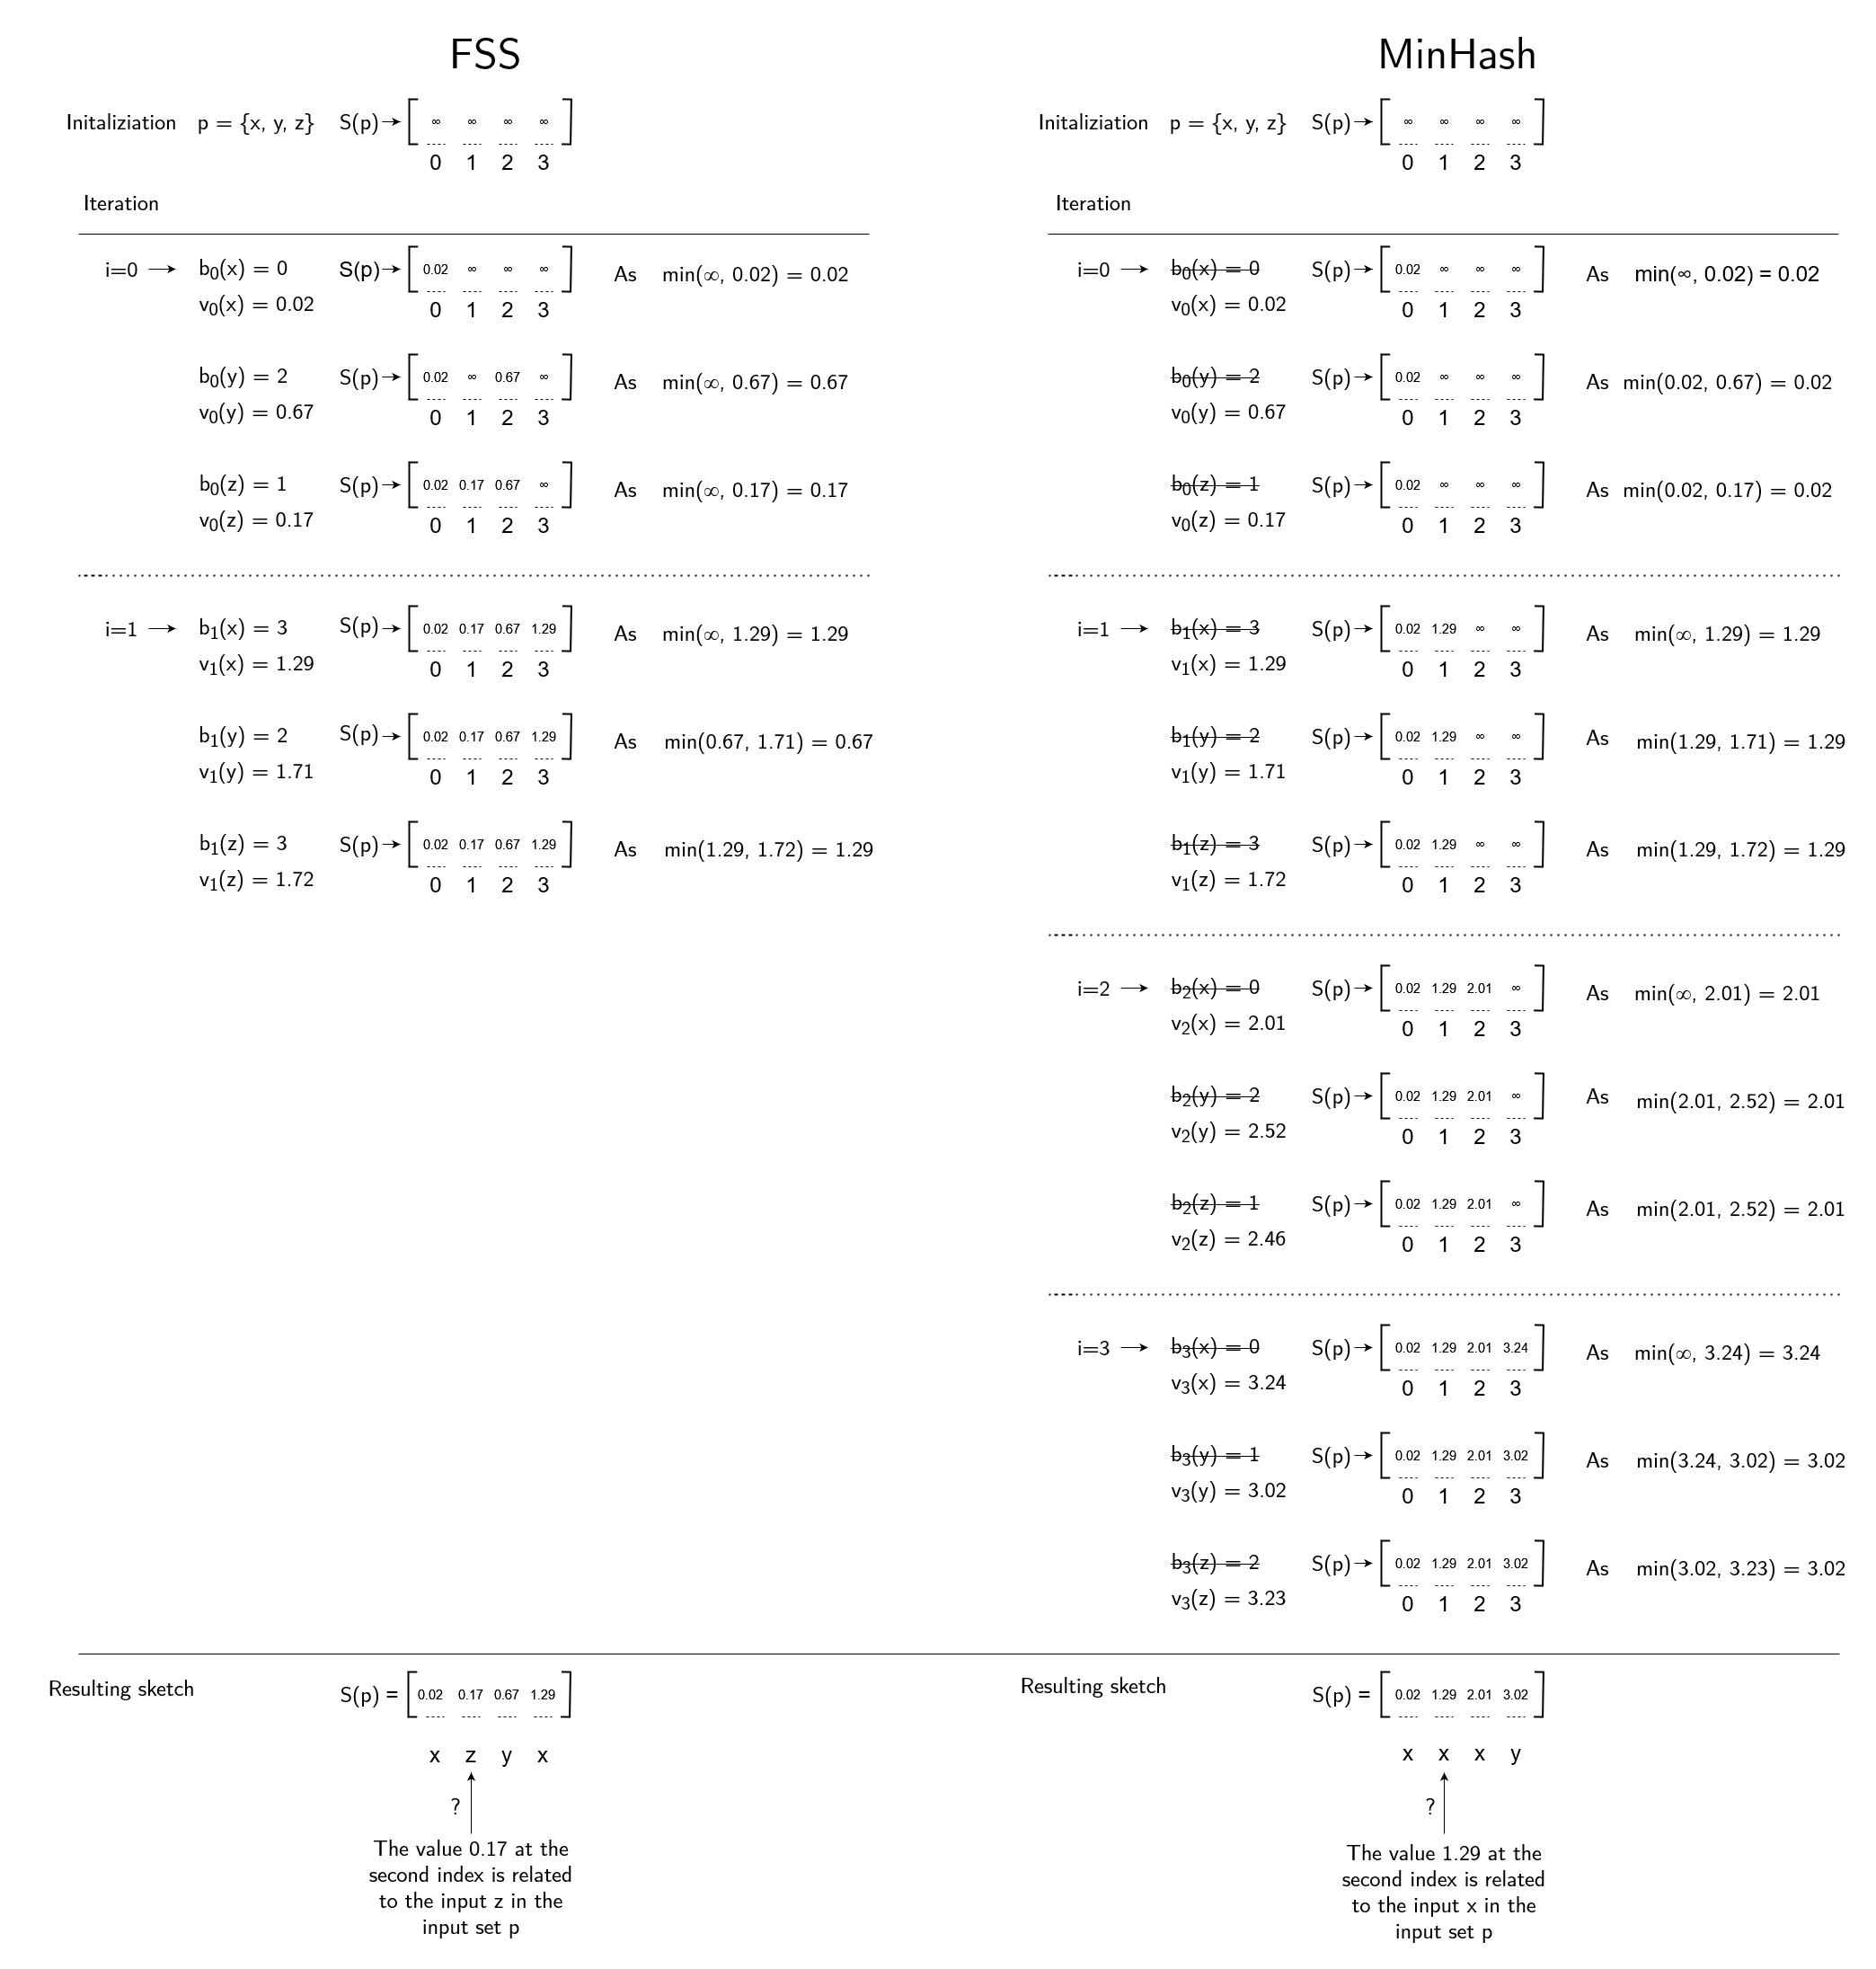
\includegraphics[width=\textwidth]{Schematic illustration FSS vs MinHash.png}
    \caption[Schematic illustration of FSS and MinHash algorithm]{\textbf{Schematic comparison of FSS and MinHash algorithm}. For FSS and MinHash we show the steps that are required for creating a sketch of length $4$ of an input $p = \{x, y, z\}$. }
    \label{fig:schematic_fss_vs_minhash}
\end{figure}

We can imagine that the discussion of FSS so far has been a bit too abstract to understand the logic behind the sketching scheme. Hence, we have created a visualization of the necessary algorithmic steps towards a sketch $S(p$) for both FSS and MinHash, which is shown in Figure \ref{fig:schematic_fss_vs_minhash}. In this example both algorithms are used to create a sketch of length $n=4$ of the input set $p=\{x, y, z\}$. We first discuss the steps that FSS takes. 

Before any iterations of the fill-sketch algorithm takes place, a sketch $S(p)$ of length $n=4$ is instantiated with all values set equal to $+\infty$. In the first iteration ($i=0$), the first hash function $h_0(\cdot)$ is applied to the first element $x$ in the input set $p$. $b_0(x) = 0 $ and $v_0(x) = 0.02$, which means that the algorithm checks whether $0.02$ is smaller than the current value in the bin with index $0$, which is $+infty$. Since that is the case, $v_0(x) = 0.02$ is placed in  $b_0(x) = 0 $. The same steps are undertaken for the elements $y$ and $z$. This leads to an intermediate sketch $S(p) = [0.02\text{  }0.17\text{  }0.67\text{  }+\infty]$ after the first iteration of the Fill-sketch algorithm. Due to the restriction that $v_i(a) \in [i, i + 1)$ as defined by Equation \ref{eq:random_hash_functions_fss},  it is certain that all elements of this intermediate version of $S(p)$ that are not equal to $+\infty$ will be part of the final sketch $S(p)$. 

In the second iteration ($i=1$), we find that $b_1(x) = 3 $ and $v_1(x)=1.29$. The bin with index $3$ still contains the value $+\infty$, which following the rules of the fill-sketch algorithm is replaced by $1.29$. Then for the element $y$, it turns out that $b_1(y)=2$ and $v_1(y) = 1.71$. The current value in the bin with index $2$ is $0.67$, which is smaller than $1.71$. Hence, this value is unchanged, showing by example that values placed in sketch bins in earlier iterations cannot be replaced in subsequent iterations. Lastly, the hash function $h_1(\cdot)$ applied to the element $z$ results in $b_1(z) = 3$ and $v_1(z) = 1.72$. The current value in the bin with index $3$ is $1.29$. Since this value is smaller than $1.72$, it is not replaced. As there is no value in the intermediate sketch $S(p) = [0.02\text{  }0.17\text{  }0.67\text{  }1.29]$ equal to $+\infty$ anymore, we know that we have reached the final version of the sketch and no subsequent iterations are necessary.

The right side of Figure \ref{fig:schematic_fss_vs_minhash} is devoted to a schematic visualization of the creation of a MinHash sketch. This algorithm is guaranteed to take four iterations to reach its goal of creating a sketch. In each iteration $i$, a random hash function $h_i(\cdot)$ is applied to the elements in $p$. The lowest resulting hash value is placed in the bin with index $i$. To easily compare FSS with MinHash, we use $v_i(\cdot)$, one of the two random hash functions used by FSS, as the random hash function $h_i(\cdot)$. Although $v_i(\cdot)$ returns a random real number instead of random integers, it still functions as a valid hash function for MinHash. 

\cite{DahlgaardKT17} prove that FSS provides unbiased estimates of the Jaccard similarity $J(p,p')$ of two sets of elements $p$ and $p'$. Furthermore the claim is made that these estimates are significantly more precise than estimates by the MinHash algorithm for a given sketch length $n$. Why would that be the case? 

MinHash uses solely \textit{sampling with replacement}: the $j$-th MinHash sketch value is equal to $\min\{v_j(a) | a \in p\}$. In other words, for the $j$-th MinHash sketch value we consider again the hash functions outputs of all elements $a \in p$. This opens up the possibility that a large part of the sketch is determined by a small subset of $p$. To an extent, such an outcome can also be observed in the example in Figure \ref{fig:schematic_fss_vs_minhash}. In the final MinHash sketch, $3$ out of $4$ elements are related to $x$, while there is no element that is related to $z$. In the most extreme case it is even possible that all elements $S$ are directly related to just one element $a \in p$. 

FSS injects an element of \textit{sampling without replacement}, which encourages a more even spread of information from $p$ into $S$. Within an iteration, distinct bins can be filled with values related to distinct elements in $p$. This can also be observed in the example in Figure \ref{fig:schematic_fss_vs_minhash}, where in the first iteration the first bin is filled with the value related to $x$, the second bin gets the value related to $z$, and the third bin receives a value related to $y$. As discussed before, these values are guaranteed to be part of the final sketch as well, due to the constraint that $\forall k > i, \forall a \in p:\text{ } v_i(a) < v_k(a)$. This approach results in a sketch $S(p)$ that is generally more representative of the input $p$ than its MinHash equivalent.

Furthermore, the authors show that their proposed algorithm for creating a single sketch of input $p$ is expected to run in $O(n\log{n} +  \vert p \vert)$, where $n$ refers to the length of the sketch. With MinHash running in $O(n * \vert p \vert)$, this implies that FSS is expected to be more efficient than MinHash, as long as $\vert p \vert > \log{n}$. These conditions are satisified in the example in Figure \ref{fig:schematic_fss_vs_minhash} as well with $\vert p \vert=3> \log{4} = 1.38$. As a consequence, FSS needs only two iterations to create a fully filled sketch $S(p)$, while MinHash requires four iterations.
%Once a value $v_i(a)$ is placed in an entry $j$ of $S$ by some hash function $h_i(a)$, then it follows from \ref{eq:definition_sketch_fss} that it won't be replaced by any $v_k(a)$ where $k > i$. 
% The claim of improved preciseness is not backed up by an experimental evaluation.

% MIX OF WITH AND WITHOUT REPLACEMENT BECAUSE WE GO THROUGH ALL a IN A every iteration, this lowers the variance of the estimate!
\subsection{Mixed tabulation hashing}
\label{subsec:mixed_tab}

To speed things up further, the random hash functions $h_i$ can be implemented using only one mixed tabulation hash function \citep{DahlgaardKRT15}, implying a very low-cost hash evaluation that runs in $O(1)$. Mixed tabulation hashing is a specific example of a larger class of tabulation hashing algorithms, which revolve around tables filled with random hashes. Depending on the value to be hashed, certain elements are retrieved from the tables, to which computationally cheap XOR operations are applied in order to obtain the hash. We have included Figure \ref{fig:schematic_mixed_tabulation_hashing}, which shows the steps taken when generating a random hash value using the mixed tabulation hashing algorithm. As a start, two tables T1 and T2 are created and filled with random values generated by a $20$-degree polynomial hash function. Both have a dimension of $256 \times 4$, but T1 is filled with $64$-bit integers, while T2 contains $32$-bit integers. In step $3$ the binary representation of $x$ is split in $c=4$ $8$-bit parts. The first part is used to pick a 64-bit element from the first column of T1, where the row is determined by its base-10 representation. The maximum $8$-bit value in base-10 is equivalent to $255$, so we are conveniently guaranteed to find an element in $T1$. The same approach is used to pick elements from the other columns in T1 in step 4. Then, as a fifth step XOR operations are applied to the retrieved elements, which results in a 64-bit integer $h$. Now, if we would be doing simple tabulation hashing, as first proposed by \cite{zobrist1970new}, this would be the final hash value. 

\begin{figure}[!htb]
    \centering
    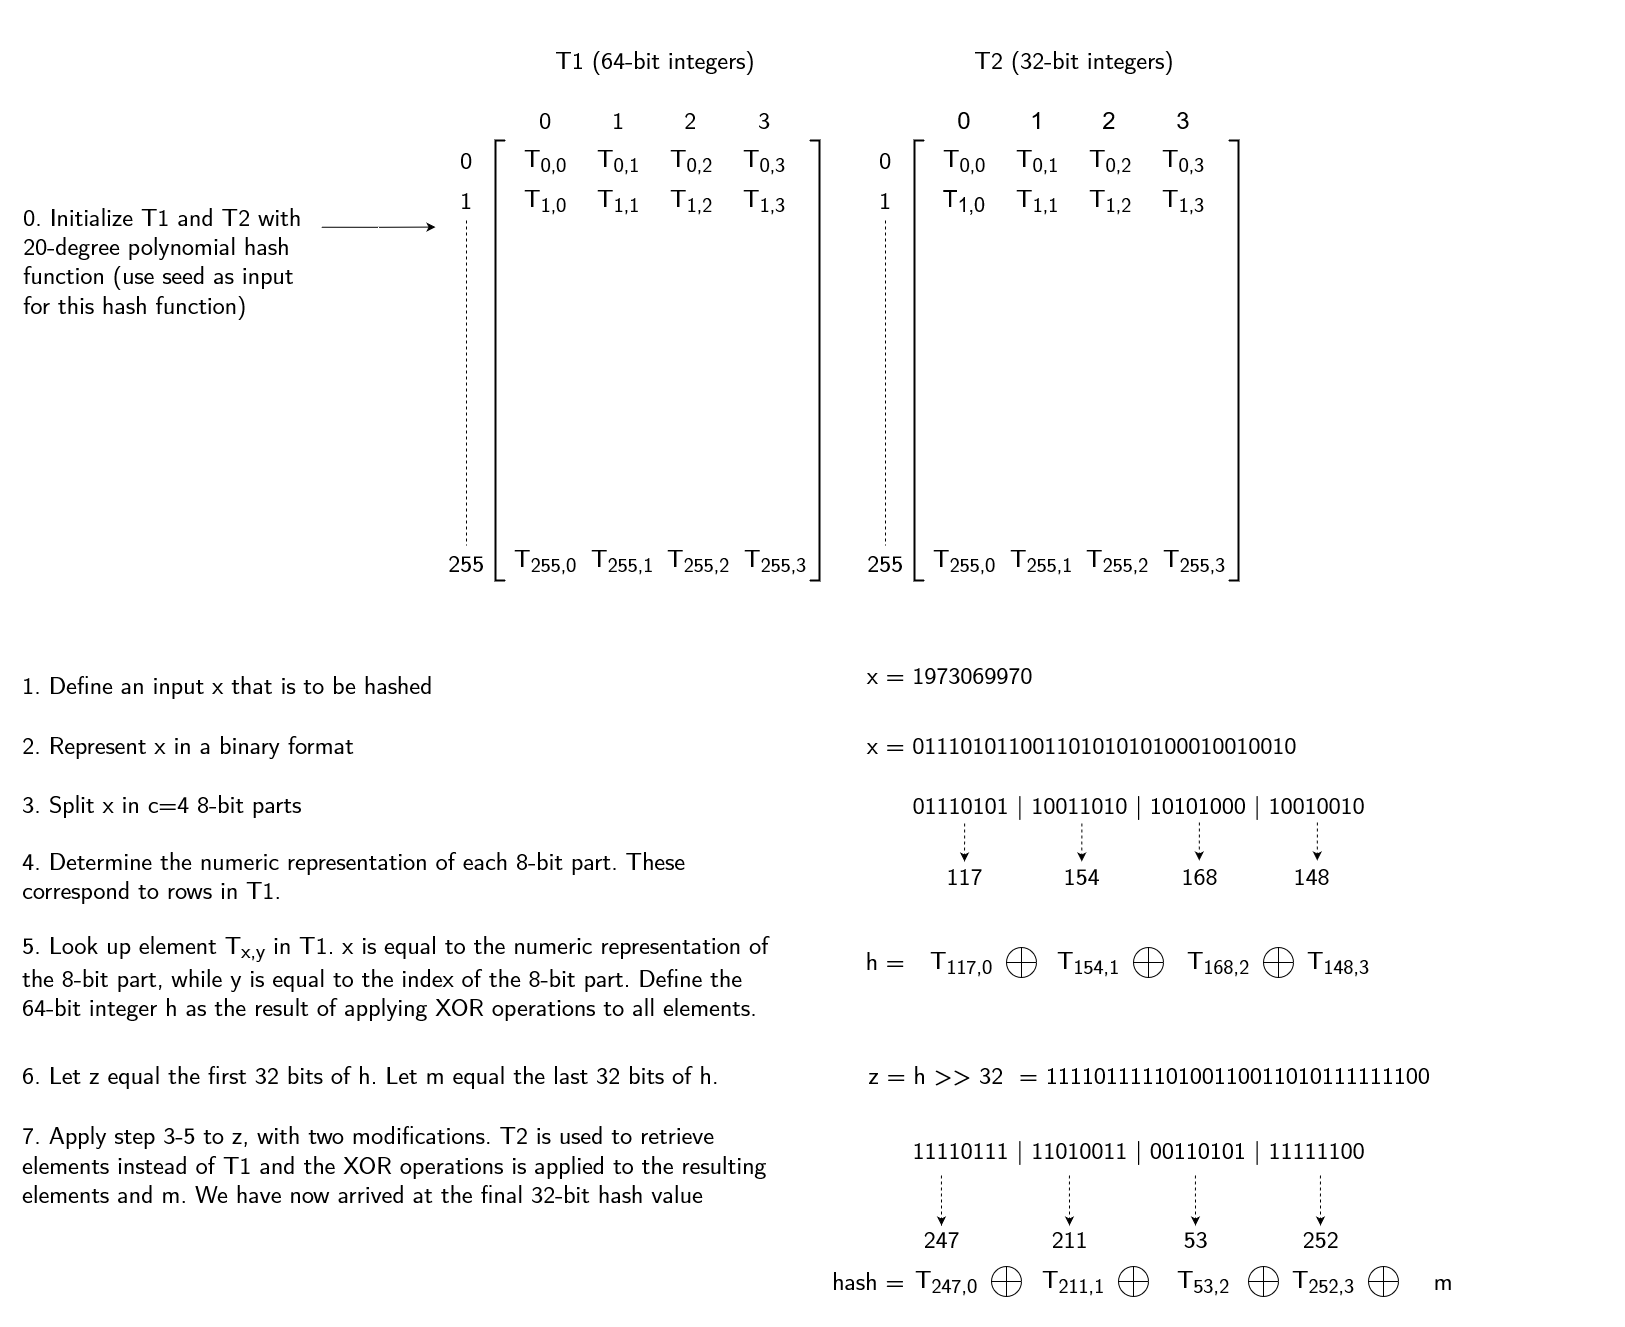
\includegraphics[width=\textwidth]{mixed_tabulation_hashing_2.png}
    \caption[Schematic illustration of mixed tabulation hashing algorithm]{\textbf{Schematic illustration of mixed tabulation hashing algorithm}.}
    \label{fig:schematic_mixed_tabulation_hashing}
\end{figure}

Mixed tabulation hashing improves on simple tabulation hashing by takings things a step further. $h$ is split in two parts. The first 32 bits are used to retrieve four 32-bit elements from $T2$ in the same manner as elements were retrieved from T1. Then the final hash value is generated by applying XOR operations to these four elements and the last 32 bits of $h$. 

\cite{DahlgaardKRT15} show that the mixed tabulation hash function has superior randomness properties compared to simple and double tabulation \citep{Thorup13} hashing approaches, while also being computationally efficient. Once the hash tables T1 and T2 are generated, inputs can be hashed at very low cost, using solely bitwise operations.



% Hence, especially for sparse datasets FSS is an attractive alternative.
%The authors make the theoretical case that their algorithm runs more efficiently when implemented in a near neighbor search compared to the original minhash method, but do not back this up with any proper experimental evaluation. 

%SOMETHING ABOUT SEPARATION ALGORITHM?
%\section{Comparing LSH approaches}
%There have been numerous studies comparing the wide range of LSH approaches out there in order to give more guidance to future researchers and practitioners on which algorithms to use under which circumstances.
% \cite{Shrivastava014} do a theoretical comparison of MinHash and SimHash in the case of binary data. They show that the resemblance similarity $R$ (Jaccard similarity) closely resembles the cosine similarity $S$ in the case of binary data. More specifically, the following bounds for $R$ will always apply:
% \begin{equation}
%     S^2 \leq R \leq \frac{S}{2 - S}
% \end{equation}
% Please note that as $S$ increases ($S \rightarrow 1$), these functions will converge, implying that a very high degree of overlap between the cosine similarity and resemblance similarity exists when applied to highly-similar inputs ($R$ and $S$ close to 1).

% When applied to the task of retrieving the top-$k$ near neighbours, for a given recall the MinHash algorithm requires to visit significantly less candidate points than the SimHash algorithm. This is the outcome in all 6 binary datasets that the algorithms are applied to. What makes this result even more interesting is that the base similarity measure that is used to define the actual closeness of data points is the cosine similarity. While evaluating their performance against the cosine similarity, they conclude that MinHash significantly outperforms SimHash when it comes to comparing highly-similar inputs. This result also holds to a lesser extent in collections where data points are less similar. 
\section{Amplification of LSH families}
\label{section:lit:amplifying}
\cite{LeskovecRU14} mention a technique to amplify $(d_1,d_2,p_1,p_2)$-sensitive families $\mathcal{H}$ so that new LSH families can be constructed that posses certain desired properties. The key idea here is too use the results of multiple hash functions to confirm or deny the similarity. They offer two pathways to achieve this.

The first pathway is to use an AND-construction. All functions that are part of the new family $\mathcal{H}'$ actually consists of $r$ functions of the original $(d_1,d_2,p_1,p_2)$-sensitive family $\mathcal{H}$. For such a function $f\in\mathcal{H}'$ we say that $f(p)=f(p')$ if and only if $f_i(p)=f_i(p')$ for all $i=1,2,...,r$. The functions $f_i$ are independently chosen from $\mathcal{H}$. As per the derivations in Equation \ref{eq:defining_families_and_constructions}, using Definition \ref{def:LSH}, it follows that $\mathcal{H}'$ is a $(d_1,d_2,p_1^r,p_2^r)$-sensitive family.

\begin{equation}
    \begin{aligned}
        &\operatorname{sim}(p, p') \geq d_1 \stackrel{\ref{def:LSH}}{\Rightarrow} \operatorname{Pr}[f_i(p)=f_i(p')] \geq p_1  \Rightarrow \operatorname{Pr}[f(p)=f(p')] = \prod_{i=1}^{r} \operatorname{Pr}[f_i(p)=f_i(p')]   \stackrel{a}{\geq} p_1^r \\
        &\operatorname{sim}(p, p') \leq d_2 \stackrel{\ref{def:LSH}}{\Rightarrow} \operatorname{Pr}[f_i(p)=f_i(p')] \leq p_2  \Rightarrow \operatorname{Pr}[f(p)=f(p')] = \prod_{i=1}^{r} \operatorname{Pr}[f_i(p)=f_i(p')]  \stackrel{b}{\leq} p_2^r
        \label{eq:defining_families_and_constructions}
    \end{aligned}
\end{equation}
where the last inequality superscripted with $a$ follows from  
\begin{equation}
    \begin{aligned}
    \operatorname{Pr}[f_i(p)=f_i(p')] &\geq p_1 \Rightarrow \\ 
    \prod_{i=1}^{r} \operatorname{Pr}[f_i(p)=f_i(p')] &\geq p_1^r 
    \end{aligned}
\end{equation}

Similar logic can be used to derive a proof for the inequality in Equation \ref{eq:defining_families_and_constructions} superscripted by $b$. 

The second pathway is to use an OR-construction. Instead of requiring all functions drawn from the original family $\mathcal{H}$ to agree, for this construction to result in a match we only need one of the functions to agree. So, for such a function $f\in\mathcal{H}'$ we say that $f(p)=f(p')$ if and only if $\exists j \in \{1,2,...,b\} \Rightarrow f_j(p)=f_j(p')$.
If we use $b$ functions $f_j(\cdot)$, then following the derivations in Equation \ref{eq:defining_families_or_constructions} we can create a $(d_1,d_2,1 - (1-p_1)^b,1-(1-p_2)^b)$-sensitive family $\mathcal{H}'$.

\begin{equation}
    \begin{aligned}
        &\operatorname{sim}(p, p') \geq d_1 \stackrel{\ref{def:LSH}}{\Rightarrow} \operatorname{Pr}[f_j(p)=f_j(p')] \geq p_1  \Rightarrow \operatorname{Pr}[f(p)=f(p')] = 1 - \prod_{j=1}^{b}( 1 -  \operatorname{Pr}[f_j(p)\neq f_j(p')] ) \stackrel{a}{\geq} 1 -  (1 -  p_1) ^ b \\
        &\operatorname{sim}(p, p') \leq d_2 \stackrel{\ref{def:LSH}}{\Rightarrow} \operatorname{Pr}[f_j(p)=f_j(p')] \leq p_2  \Rightarrow \operatorname{Pr}[f(p)=f(p')] = 1 - \prod_{j=1}^{b}( 1 -  \operatorname{Pr}[f_j(p)\neq f_i(p')] ) \stackrel{b}{\leq} 1 -  (1 -  p_2) ^ b 
        \label{eq:defining_families_or_constructions}
    \end{aligned}
\end{equation}

where the last inequality superscripted with $a$ follows from 

\begin{equation}
    \begin{aligned}
    \operatorname{Pr}[f_i(p)=f_i(p')] &\geq p_1 \Leftrightarrow \\
    1 - \operatorname{Pr}[f_i(p)=f_i(p')] &\leq 1 -  p_1 \Rightarrow \\ 
    \prod_{i=1}^{b}(1 - \operatorname{Pr}[f_i(p)=f_i(p')]) &\leq (1 -  p_1) ^ b \Leftrightarrow \\ 
    1 -  \prod_{i=1}^{b}(1 - \operatorname{Pr}[f_i(p)=f_i(p')]) &\geq 1 -  (1 -  p_1) ^ b  
    \end{aligned}
    \label{eq:proof_or_constructions}
\end{equation}

Again, similar logic as applied in Equation \ref{eq:proof_or_constructions} can be used to derive a proof for the inequality in Equation \ref{eq:defining_families_or_constructions} superscripted by $b$.

The AND and OR construction have an opposing effect. The AND-construction lower $p_1$ and $p_2$, while the OR-constructions increase $p_1$ and $p_2$. By applying them iteratively, it might be possible to create families that accept dissimilar items with a lower probability ($p_2 \rightarrow 0$), while accepting similar items at a preferred higher probability ($p_1 \rightarrow 1$). As this decreases the $\rho$ measure as shown in Section \ref{section:lit:introducing_lsh}, more specifically Equation \ref{eq:partial_derivatives_rho}, we obtain a more effective LSH scheme. \cite{LeskovecRU14} show by example that this is the case for the amplified  $(d_1,d_2, 1 -  (1 - p_1^r) ^ b, 1 -  (1 -  p_2^r) ^ b )$-sensitive family $\mathcal{H}'$, obtained by first applying $r$ AND-constructions and then $b$ OR-constructions, compared to the original $(d_1,d_2,p_1,p_2)$-sensitive family $\mathcal{H}$. However, we must also note that $\mathcal{H}'$  requires $b*r$ as many hash functions as $\mathcal{H}$. The question remains if $\mathcal{H}'$ is also able to deliver increased effectiveness compared to arbitrary traditional LSH families $\mathcal{G}$ which use as many hash function inputs as $\mathcal{H}'$. To this day, we do not find a successful effort in the literature which is able to show this. 

Manipulating parameters $b$ and $r$ can be compared to manipulating the $b$ and $r$ in the original implementation (see \ref{eq:s_curve}). For example, if we start with $256 = 16^2$ LSH functions $f_i$, then we could use AND and OR constructions in the following way to mimic a traditional LSH scheme. We split the functions into $16$ sets that each contain $16$ functions $f_i$. Within each set, equivalent to buckets in the traditional scheme, we apply the AND-construction. To the result of each set we apply the OR-construction. In order to define this method mathematically, it helps to define the following function
\begin{equation}
    h_i(x,y) = \begin{cases} 1 \text{          , if} f_i(p) = f_i(p')\\
    0 \text{         , otherwise}
    \end{cases}
\end{equation}
We can define an output function $o(x,y)$, which mimics the behavior of the scheme described above, as
\begin{equation}
    o(p,p') = \min\{\sum_{b=1}^{16}\prod_{r=1}^{16}h_{b \cdot r}(p,p'),1\}
\end{equation}
If $o(p,p') = 1$, the scheme considers $(p,p')$ as a candidate pair. It is obvious that this is the exact same behavior as a traditional LSH scheme with $b$ buckets and $r$ hash functions in each bucket. What is interesting though, is that the AND/OR-constructions allow us to build more complex versions of LSH schemes. 

For example, we could split the same set of $256 = 4^4$ functions into sets of size $4$. Within each set of $4$ functions we apply the AND-construction, after which we apply the OR-construction to groups of $4$ sets. So, we have $16$ functions $g_j$, for which we know that
\begin{equation}
    g_j(p, p') =  \min\{\sum_{b_1=1}^{4}\prod_{r_1=1}^{4}h_{b_1 \cdot r_1 \cdot j}(p,p'),1\} \text{  for } j \in \{1,...,16\}
\end{equation}
 We can again split these functions in sets of size $4$, to which we iteratively apply an AND-construction and an OR-construction, such that we define the output function $o(p,p')$ as 
\begin{equation}
    o(p,p') = \min\{\sum_{b_2=1}^{4}\prod_{r_2=1}^{4}g_{b_2 \cdot r_2}(p,p'),1\}
\end{equation} 
Again, if $o(p,p') = 1$, this scheme considers $x$ and $y$ as candidate pairs.

We conclude that it is not only possible to use AND/OR-constructions to create a scheme that behaves exactly like traditional LSH schemes, but that it also allows for more complex schemes which potentially possess advantageous properites. In that sense one could argue that schemes with AND/OR-constructions can be regarded as a generalization to the traditional LSH scheme.